% Created by tikzDevice version 0.12.6 on 2025-04-16 10:40:02
% !TEX encoding = UTF-8 Unicode
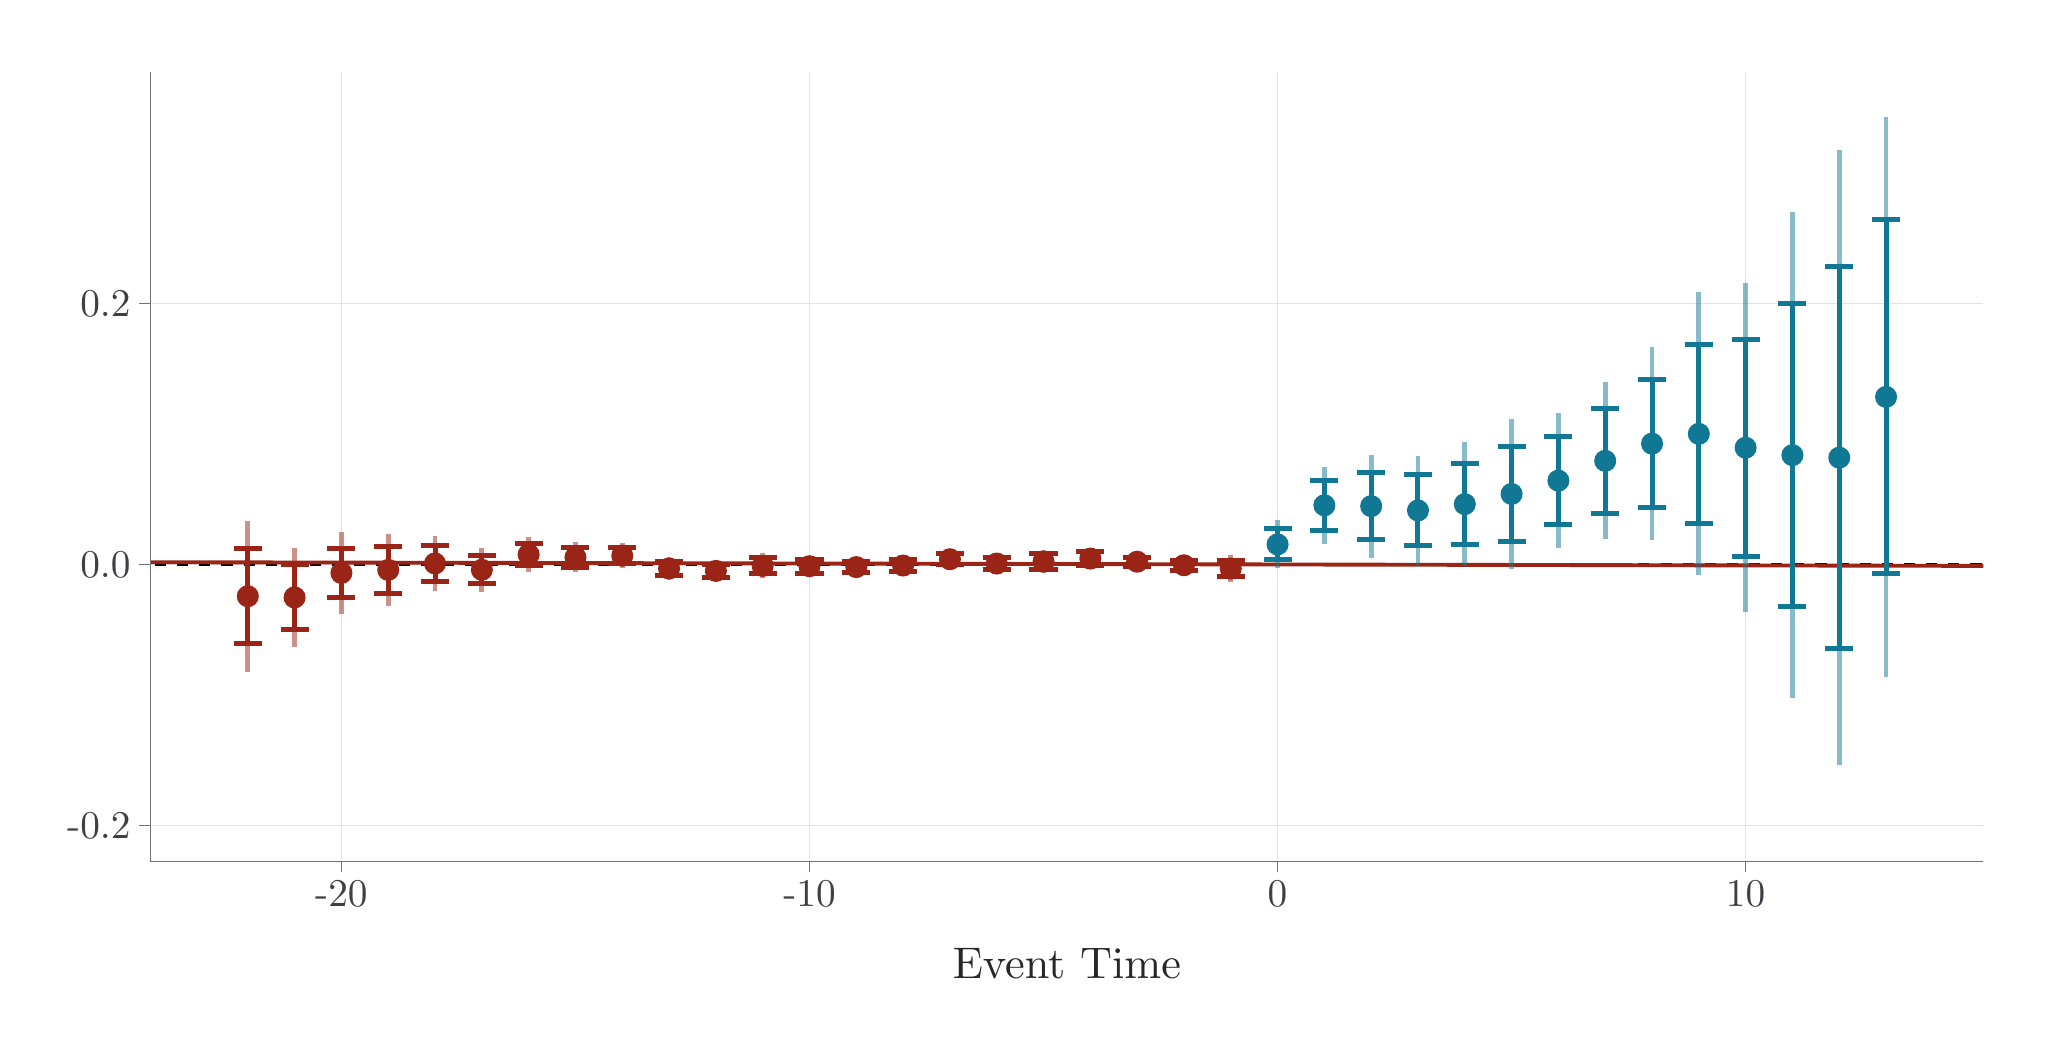
\begin{tikzpicture}[x=1pt,y=1pt]
\definecolor{fillColor}{RGB}{255,255,255}
\path[use as bounding box,fill=fillColor] (0,0) rectangle (722.70,361.35);
\begin{scope}
\path[clip] (  0.00,  0.00) rectangle (722.70,361.35);
\definecolor{drawColor}{RGB}{255,255,255}

\path[draw=drawColor,line width= 0.8pt,line join=round,line cap=round,fill=fillColor] (  0.00,  0.00) rectangle (722.70,361.35);
\end{scope}
\begin{scope}
\path[clip] ( 44.36, 60.16) rectangle (706.70,345.35);
\definecolor{drawColor}{RGB}{255,255,255}
\definecolor{fillColor}{RGB}{255,255,255}

\path[draw=drawColor,line width= 0.8pt,line join=round,line cap=round,fill=fillColor] ( 44.36, 60.16) rectangle (706.70,345.35);
\definecolor{drawColor}{RGB}{228,228,231}

\path[draw=drawColor,line width= 0.4pt,line join=round] ( 44.36, 73.12) --
	(706.70, 73.12);

\path[draw=drawColor,line width= 0.4pt,line join=round] ( 44.36,167.40) --
	(706.70,167.40);

\path[draw=drawColor,line width= 0.4pt,line join=round] ( 44.36,261.68) --
	(706.70,261.68);

\path[draw=drawColor,line width= 0.4pt,line join=round] (113.37, 60.16) --
	(113.37,345.35);

\path[draw=drawColor,line width= 0.4pt,line join=round] (282.50, 60.16) --
	(282.50,345.35);

\path[draw=drawColor,line width= 0.4pt,line join=round] (451.64, 60.16) --
	(451.64,345.35);

\path[draw=drawColor,line width= 0.4pt,line join=round] (620.78, 60.16) --
	(620.78,345.35);
\definecolor{drawColor}{RGB}{0,0,0}

\path[draw=drawColor,line width= 0.9pt,dash pattern=on 4pt off 4pt ,line join=round] (-617.98,167.40) -- (1369.04,167.40);
\definecolor{drawColor}{RGB}{154,36,21}

\path[draw=drawColor,line width= 1.4pt,line join=round] (-617.98,169.54) -- (1369.04,165.52);
\definecolor{drawColor}{RGB}{154,36,21}

\path[draw=drawColor,draw opacity=0.50,line width= 1.7pt,line join=round] ( 79.54,128.65) -- ( 79.54,183.16);

\path[draw=drawColor,draw opacity=0.50,line width= 1.7pt,line join=round] ( 96.45,137.44) -- ( 96.45,173.49);

\path[draw=drawColor,draw opacity=0.50,line width= 1.7pt,line join=round] (113.37,149.64) -- (113.37,178.99);

\path[draw=drawColor,draw opacity=0.50,line width= 1.7pt,line join=round] (130.28,152.36) -- (130.28,178.46);

\path[draw=drawColor,draw opacity=0.50,line width= 1.7pt,line join=round] (147.19,157.72) -- (147.19,177.76);

\path[draw=drawColor,draw opacity=0.50,line width= 1.7pt,line join=round] (164.11,157.43) -- (164.11,173.47);

\path[draw=drawColor,draw opacity=0.50,line width= 1.7pt,line join=round] (181.02,164.79) -- (181.02,177.19);

\path[draw=drawColor,draw opacity=0.50,line width= 1.7pt,line join=round] (197.94,164.55) -- (197.94,175.36);

\path[draw=drawColor,draw opacity=0.50,line width= 1.7pt,line join=round] (214.85,165.95) -- (214.85,175.14);

\path[draw=drawColor,draw opacity=0.50,line width= 1.7pt,line join=round] (231.76,161.77) -- (231.76,170.09);

\path[draw=drawColor,draw opacity=0.50,line width= 1.7pt,line join=round] (248.68,161.53) -- (248.68,168.57);

\path[draw=drawColor,draw opacity=0.50,line width= 1.7pt,line join=round] (265.59,162.32) -- (265.59,171.40);

\path[draw=drawColor,draw opacity=0.50,line width= 1.7pt,line join=round] (282.50,163.05) -- (282.50,170.45);

\path[draw=drawColor,draw opacity=0.50,line width= 1.7pt,line join=round] (299.42,163.31) -- (299.42,169.53);

\path[draw=drawColor,draw opacity=0.50,line width= 1.7pt,line join=round] (316.33,163.66) -- (316.33,170.33);

\path[draw=drawColor,draw opacity=0.50,line width= 1.7pt,line join=round] (333.25,166.08) -- (333.25,172.46);

\path[draw=drawColor,draw opacity=0.50,line width= 1.7pt,line join=round] (350.16,164.40) -- (350.16,171.02);

\path[draw=drawColor,draw opacity=0.50,line width= 1.7pt,line join=round] (367.07,164.16) -- (367.07,172.69);

\path[draw=drawColor,draw opacity=0.50,line width= 1.7pt,line join=round] (383.99,166.06) -- (383.99,172.97);

\path[draw=drawColor,draw opacity=0.50,line width= 1.7pt,line join=round] (400.90,165.77) -- (400.90,170.97);

\path[draw=drawColor,draw opacity=0.50,line width= 1.7pt,line join=round] (417.81,164.20) -- (417.81,169.97);

\path[draw=drawColor,draw opacity=0.50,line width= 1.7pt,line join=round] (434.73,161.16) -- (434.73,170.64);
\definecolor{drawColor}{RGB}{16,120,149}

\path[draw=drawColor,draw opacity=0.50,line width= 1.7pt,line join=round] (451.64,165.98) -- (451.64,183.29);

\path[draw=drawColor,draw opacity=0.50,line width= 1.7pt,line join=round] (468.56,174.90) -- (468.56,202.61);

\path[draw=drawColor,draw opacity=0.50,line width= 1.7pt,line join=round] (485.47,169.88) -- (485.47,207.04);

\path[draw=drawColor,draw opacity=0.50,line width= 1.7pt,line join=round] (502.38,167.14) -- (502.38,206.66);

\path[draw=drawColor,draw opacity=0.50,line width= 1.7pt,line join=round] (519.30,166.76) -- (519.30,211.62);

\path[draw=drawColor,draw opacity=0.50,line width= 1.7pt,line join=round] (536.21,165.83) -- (536.21,219.89);

\path[draw=drawColor,draw opacity=0.50,line width= 1.7pt,line join=round] (553.12,173.38) -- (553.12,221.95);

\path[draw=drawColor,draw opacity=0.50,line width= 1.7pt,line join=round] (570.04,176.49) -- (570.04,233.17);

\path[draw=drawColor,draw opacity=0.50,line width= 1.7pt,line join=round] (586.95,176.13) -- (586.95,245.94);

\path[draw=drawColor,draw opacity=0.50,line width= 1.7pt,line join=round] (603.86,163.41) -- (603.86,265.76);

\path[draw=drawColor,draw opacity=0.50,line width= 1.7pt,line join=round] (620.78,150.22) -- (620.78,268.92);

\path[draw=drawColor,draw opacity=0.50,line width= 1.7pt,line join=round] (637.69,118.95) -- (637.69,294.81);

\path[draw=drawColor,draw opacity=0.50,line width= 1.7pt,line join=round] (654.61, 94.83) -- (654.61,317.13);

\path[draw=drawColor,draw opacity=0.50,line width= 1.7pt,line join=round] (671.52,126.64) -- (671.52,329.21);
\definecolor{drawColor}{RGB}{154,36,21}

\path[draw=drawColor,line width= 1.8pt,line join=round] ( 74.47,173.07) --
	( 84.61,173.07);

\path[draw=drawColor,line width= 1.8pt,line join=round] ( 79.54,173.07) --
	( 79.54,138.74);

\path[draw=drawColor,line width= 1.8pt,line join=round] ( 74.47,138.74) --
	( 84.61,138.74);

\path[draw=drawColor,line width= 1.8pt,line join=round] ( 91.38,167.22) --
	(101.53,167.22);

\path[draw=drawColor,line width= 1.8pt,line join=round] ( 96.45,167.22) --
	( 96.45,143.71);

\path[draw=drawColor,line width= 1.8pt,line join=round] ( 91.38,143.71) --
	(101.53,143.71);

\path[draw=drawColor,line width= 1.8pt,line join=round] (108.29,173.14) --
	(118.44,173.14);

\path[draw=drawColor,line width= 1.8pt,line join=round] (113.37,173.14) --
	(113.37,155.48);

\path[draw=drawColor,line width= 1.8pt,line join=round] (108.29,155.48) --
	(118.44,155.48);

\path[draw=drawColor,line width= 1.8pt,line join=round] (125.21,173.99) --
	(135.36,173.99);

\path[draw=drawColor,line width= 1.8pt,line join=round] (130.28,173.99) --
	(130.28,156.83);

\path[draw=drawColor,line width= 1.8pt,line join=round] (125.21,156.83) --
	(135.36,156.83);

\path[draw=drawColor,line width= 1.8pt,line join=round] (142.12,174.27) --
	(152.27,174.27);

\path[draw=drawColor,line width= 1.8pt,line join=round] (147.19,174.27) --
	(147.19,161.21);

\path[draw=drawColor,line width= 1.8pt,line join=round] (142.12,161.21) --
	(152.27,161.21);

\path[draw=drawColor,line width= 1.8pt,line join=round] (159.03,170.45) --
	(169.18,170.45);

\path[draw=drawColor,line width= 1.8pt,line join=round] (164.11,170.45) --
	(164.11,160.45);

\path[draw=drawColor,line width= 1.8pt,line join=round] (159.03,160.45) --
	(169.18,160.45);

\path[draw=drawColor,line width= 1.8pt,line join=round] (175.95,175.00) --
	(186.10,175.00);

\path[draw=drawColor,line width= 1.8pt,line join=round] (181.02,175.00) --
	(181.02,166.97);

\path[draw=drawColor,line width= 1.8pt,line join=round] (175.95,166.97) --
	(186.10,166.97);

\path[draw=drawColor,line width= 1.8pt,line join=round] (192.86,173.51) --
	(203.01,173.51);

\path[draw=drawColor,line width= 1.8pt,line join=round] (197.94,173.51) --
	(197.94,166.39);

\path[draw=drawColor,line width= 1.8pt,line join=round] (192.86,166.39) --
	(203.01,166.39);

\path[draw=drawColor,line width= 1.8pt,line join=round] (209.78,173.44) --
	(219.92,173.44);

\path[draw=drawColor,line width= 1.8pt,line join=round] (214.85,173.44) --
	(214.85,167.66);

\path[draw=drawColor,line width= 1.8pt,line join=round] (209.78,167.66) --
	(219.92,167.66);

\path[draw=drawColor,line width= 1.8pt,line join=round] (226.69,168.52) --
	(236.84,168.52);

\path[draw=drawColor,line width= 1.8pt,line join=round] (231.76,168.52) --
	(231.76,163.34);

\path[draw=drawColor,line width= 1.8pt,line join=round] (226.69,163.34) --
	(236.84,163.34);

\path[draw=drawColor,line width= 1.8pt,line join=round] (243.60,167.29) --
	(253.75,167.29);

\path[draw=drawColor,line width= 1.8pt,line join=round] (248.68,167.29) --
	(248.68,162.81);

\path[draw=drawColor,line width= 1.8pt,line join=round] (243.60,162.81) --
	(253.75,162.81);

\path[draw=drawColor,line width= 1.8pt,line join=round] (260.52,169.72) --
	(270.66,169.72);

\path[draw=drawColor,line width= 1.8pt,line join=round] (265.59,169.72) --
	(265.59,163.99);

\path[draw=drawColor,line width= 1.8pt,line join=round] (260.52,163.99) --
	(270.66,163.99);

\path[draw=drawColor,line width= 1.8pt,line join=round] (277.43,169.23) --
	(287.58,169.23);

\path[draw=drawColor,line width= 1.8pt,line join=round] (282.50,169.23) --
	(282.50,164.28);

\path[draw=drawColor,line width= 1.8pt,line join=round] (277.43,164.28) --
	(287.58,164.28);

\path[draw=drawColor,line width= 1.8pt,line join=round] (294.34,168.43) --
	(304.49,168.43);

\path[draw=drawColor,line width= 1.8pt,line join=round] (299.42,168.43) --
	(299.42,164.41);

\path[draw=drawColor,line width= 1.8pt,line join=round] (294.34,164.41) --
	(304.49,164.41);

\path[draw=drawColor,line width= 1.8pt,line join=round] (311.26,169.12) --
	(321.41,169.12);

\path[draw=drawColor,line width= 1.8pt,line join=round] (316.33,169.12) --
	(316.33,164.88);

\path[draw=drawColor,line width= 1.8pt,line join=round] (311.26,164.88) --
	(321.41,164.88);

\path[draw=drawColor,line width= 1.8pt,line join=round] (328.17,171.35) --
	(338.32,171.35);

\path[draw=drawColor,line width= 1.8pt,line join=round] (333.25,171.35) --
	(333.25,167.19);

\path[draw=drawColor,line width= 1.8pt,line join=round] (328.17,167.19) --
	(338.32,167.19);

\path[draw=drawColor,line width= 1.8pt,line join=round] (345.08,169.85) --
	(355.23,169.85);

\path[draw=drawColor,line width= 1.8pt,line join=round] (350.16,169.85) --
	(350.16,165.58);

\path[draw=drawColor,line width= 1.8pt,line join=round] (345.08,165.58) --
	(355.23,165.58);

\path[draw=drawColor,line width= 1.8pt,line join=round] (362.00,171.29) --
	(372.15,171.29);

\path[draw=drawColor,line width= 1.8pt,line join=round] (367.07,171.29) --
	(367.07,165.56);

\path[draw=drawColor,line width= 1.8pt,line join=round] (362.00,165.56) --
	(372.15,165.56);

\path[draw=drawColor,line width= 1.8pt,line join=round] (378.91,171.91) --
	(389.06,171.91);

\path[draw=drawColor,line width= 1.8pt,line join=round] (383.99,171.91) --
	(383.99,167.12);

\path[draw=drawColor,line width= 1.8pt,line join=round] (378.91,167.12) --
	(389.06,167.12);

\path[draw=drawColor,line width= 1.8pt,line join=round] (395.83,170.05) --
	(405.97,170.05);

\path[draw=drawColor,line width= 1.8pt,line join=round] (400.90,170.05) --
	(400.90,166.69);

\path[draw=drawColor,line width= 1.8pt,line join=round] (395.83,166.69) --
	(405.97,166.69);

\path[draw=drawColor,line width= 1.8pt,line join=round] (412.74,168.92) --
	(422.89,168.92);

\path[draw=drawColor,line width= 1.8pt,line join=round] (417.81,168.92) --
	(417.81,165.25);

\path[draw=drawColor,line width= 1.8pt,line join=round] (412.74,165.25) --
	(422.89,165.25);

\path[draw=drawColor,line width= 1.8pt,line join=round] (429.65,168.88) --
	(439.80,168.88);

\path[draw=drawColor,line width= 1.8pt,line join=round] (434.73,168.88) --
	(434.73,162.92);

\path[draw=drawColor,line width= 1.8pt,line join=round] (429.65,162.92) --
	(439.80,162.92);
\definecolor{drawColor}{RGB}{16,120,149}

\path[draw=drawColor,line width= 1.8pt,line join=round] (446.57,180.26) --
	(456.72,180.26);

\path[draw=drawColor,line width= 1.8pt,line join=round] (451.64,180.26) --
	(451.64,169.01);

\path[draw=drawColor,line width= 1.8pt,line join=round] (446.57,169.01) --
	(456.72,169.01);

\path[draw=drawColor,line width= 1.8pt,line join=round] (463.48,197.85) --
	(473.63,197.85);

\path[draw=drawColor,line width= 1.8pt,line join=round] (468.56,197.85) --
	(468.56,179.66);

\path[draw=drawColor,line width= 1.8pt,line join=round] (463.48,179.66) --
	(473.63,179.66);

\path[draw=drawColor,line width= 1.8pt,line join=round] (480.39,200.53) --
	(490.54,200.53);

\path[draw=drawColor,line width= 1.8pt,line join=round] (485.47,200.53) --
	(485.47,176.39);

\path[draw=drawColor,line width= 1.8pt,line join=round] (480.39,176.39) --
	(490.54,176.39);

\path[draw=drawColor,line width= 1.8pt,line join=round] (497.31,199.71) --
	(507.46,199.71);

\path[draw=drawColor,line width= 1.8pt,line join=round] (502.38,199.71) --
	(502.38,174.09);

\path[draw=drawColor,line width= 1.8pt,line join=round] (497.31,174.09) --
	(507.46,174.09);

\path[draw=drawColor,line width= 1.8pt,line join=round] (514.22,203.93) --
	(524.37,203.93);

\path[draw=drawColor,line width= 1.8pt,line join=round] (519.30,203.93) --
	(519.30,174.45);

\path[draw=drawColor,line width= 1.8pt,line join=round] (514.22,174.45) --
	(524.37,174.45);

\path[draw=drawColor,line width= 1.8pt,line join=round] (531.14,210.18) --
	(541.28,210.18);

\path[draw=drawColor,line width= 1.8pt,line join=round] (536.21,210.18) --
	(536.21,175.54);

\path[draw=drawColor,line width= 1.8pt,line join=round] (531.14,175.54) --
	(541.28,175.54);

\path[draw=drawColor,line width= 1.8pt,line join=round] (548.05,213.53) --
	(558.20,213.53);

\path[draw=drawColor,line width= 1.8pt,line join=round] (553.12,213.53) --
	(553.12,181.80);

\path[draw=drawColor,line width= 1.8pt,line join=round] (548.05,181.80) --
	(558.20,181.80);

\path[draw=drawColor,line width= 1.8pt,line join=round] (564.96,223.76) --
	(575.11,223.76);

\path[draw=drawColor,line width= 1.8pt,line join=round] (570.04,223.76) --
	(570.04,185.90);

\path[draw=drawColor,line width= 1.8pt,line join=round] (564.96,185.90) --
	(575.11,185.90);

\path[draw=drawColor,line width= 1.8pt,line join=round] (581.88,234.18) --
	(592.03,234.18);

\path[draw=drawColor,line width= 1.8pt,line join=round] (586.95,234.18) --
	(586.95,187.90);

\path[draw=drawColor,line width= 1.8pt,line join=round] (581.88,187.90) --
	(592.03,187.90);

\path[draw=drawColor,line width= 1.8pt,line join=round] (598.79,247.00) --
	(608.94,247.00);

\path[draw=drawColor,line width= 1.8pt,line join=round] (603.86,247.00) --
	(603.86,182.16);

\path[draw=drawColor,line width= 1.8pt,line join=round] (598.79,182.16) --
	(608.94,182.16);

\path[draw=drawColor,line width= 1.8pt,line join=round] (615.70,248.72) --
	(625.85,248.72);

\path[draw=drawColor,line width= 1.8pt,line join=round] (620.78,248.72) --
	(620.78,170.42);

\path[draw=drawColor,line width= 1.8pt,line join=round] (615.70,170.42) --
	(625.85,170.42);

\path[draw=drawColor,line width= 1.8pt,line join=round] (632.62,261.74) --
	(642.77,261.74);

\path[draw=drawColor,line width= 1.8pt,line join=round] (637.69,261.74) --
	(637.69,152.02);

\path[draw=drawColor,line width= 1.8pt,line join=round] (632.62,152.02) --
	(642.77,152.02);

\path[draw=drawColor,line width= 1.8pt,line join=round] (649.53,275.11) --
	(659.68,275.11);

\path[draw=drawColor,line width= 1.8pt,line join=round] (654.61,275.11) --
	(654.61,136.86);

\path[draw=drawColor,line width= 1.8pt,line join=round] (649.53,136.86) --
	(659.68,136.86);

\path[draw=drawColor,line width= 1.8pt,line join=round] (666.45,291.88) --
	(676.59,291.88);

\path[draw=drawColor,line width= 1.8pt,line join=round] (671.52,291.88) --
	(671.52,163.97);

\path[draw=drawColor,line width= 1.8pt,line join=round] (666.45,163.97) --
	(676.59,163.97);
\definecolor{drawColor}{RGB}{154,36,21}
\definecolor{fillColor}{RGB}{154,36,21}

\path[draw=drawColor,line width= 0.5pt,line join=round,line cap=round,fill=fillColor] ( 79.54,155.90) circle (  3.73);

\path[draw=drawColor,line width= 0.5pt,line join=round,line cap=round,fill=fillColor] ( 96.45,155.47) circle (  3.73);

\path[draw=drawColor,line width= 0.5pt,line join=round,line cap=round,fill=fillColor] (113.37,164.31) circle (  3.73);

\path[draw=drawColor,line width= 0.5pt,line join=round,line cap=round,fill=fillColor] (130.28,165.41) circle (  3.73);

\path[draw=drawColor,line width= 0.5pt,line join=round,line cap=round,fill=fillColor] (147.19,167.74) circle (  3.73);

\path[draw=drawColor,line width= 0.5pt,line join=round,line cap=round,fill=fillColor] (164.11,165.45) circle (  3.73);

\path[draw=drawColor,line width= 0.5pt,line join=round,line cap=round,fill=fillColor] (181.02,170.99) circle (  3.73);

\path[draw=drawColor,line width= 0.5pt,line join=round,line cap=round,fill=fillColor] (197.94,169.95) circle (  3.73);

\path[draw=drawColor,line width= 0.5pt,line join=round,line cap=round,fill=fillColor] (214.85,170.55) circle (  3.73);

\path[draw=drawColor,line width= 0.5pt,line join=round,line cap=round,fill=fillColor] (231.76,165.93) circle (  3.73);

\path[draw=drawColor,line width= 0.5pt,line join=round,line cap=round,fill=fillColor] (248.68,165.05) circle (  3.73);

\path[draw=drawColor,line width= 0.5pt,line join=round,line cap=round,fill=fillColor] (265.59,166.86) circle (  3.73);

\path[draw=drawColor,line width= 0.5pt,line join=round,line cap=round,fill=fillColor] (282.50,166.75) circle (  3.73);

\path[draw=drawColor,line width= 0.5pt,line join=round,line cap=round,fill=fillColor] (299.42,166.42) circle (  3.73);

\path[draw=drawColor,line width= 0.5pt,line join=round,line cap=round,fill=fillColor] (316.33,167.00) circle (  3.73);

\path[draw=drawColor,line width= 0.5pt,line join=round,line cap=round,fill=fillColor] (333.25,169.27) circle (  3.73);

\path[draw=drawColor,line width= 0.5pt,line join=round,line cap=round,fill=fillColor] (350.16,167.71) circle (  3.73);

\path[draw=drawColor,line width= 0.5pt,line join=round,line cap=round,fill=fillColor] (367.07,168.42) circle (  3.73);

\path[draw=drawColor,line width= 0.5pt,line join=round,line cap=round,fill=fillColor] (383.99,169.51) circle (  3.73);

\path[draw=drawColor,line width= 0.5pt,line join=round,line cap=round,fill=fillColor] (400.90,168.37) circle (  3.73);

\path[draw=drawColor,line width= 0.5pt,line join=round,line cap=round,fill=fillColor] (417.81,167.09) circle (  3.73);

\path[draw=drawColor,line width= 0.5pt,line join=round,line cap=round,fill=fillColor] (434.73,165.90) circle (  3.73);
\definecolor{drawColor}{RGB}{16,120,149}
\definecolor{fillColor}{RGB}{16,120,149}

\path[draw=drawColor,line width= 0.5pt,line join=round,line cap=round,fill=fillColor] (451.64,174.63) circle (  3.73);

\path[draw=drawColor,line width= 0.5pt,line join=round,line cap=round,fill=fillColor] (468.56,188.75) circle (  3.73);

\path[draw=drawColor,line width= 0.5pt,line join=round,line cap=round,fill=fillColor] (485.47,188.46) circle (  3.73);

\path[draw=drawColor,line width= 0.5pt,line join=round,line cap=round,fill=fillColor] (502.38,186.90) circle (  3.73);

\path[draw=drawColor,line width= 0.5pt,line join=round,line cap=round,fill=fillColor] (519.30,189.19) circle (  3.73);

\path[draw=drawColor,line width= 0.5pt,line join=round,line cap=round,fill=fillColor] (536.21,192.86) circle (  3.73);

\path[draw=drawColor,line width= 0.5pt,line join=round,line cap=round,fill=fillColor] (553.12,197.67) circle (  3.73);

\path[draw=drawColor,line width= 0.5pt,line join=round,line cap=round,fill=fillColor] (570.04,204.83) circle (  3.73);

\path[draw=drawColor,line width= 0.5pt,line join=round,line cap=round,fill=fillColor] (586.95,211.04) circle (  3.73);

\path[draw=drawColor,line width= 0.5pt,line join=round,line cap=round,fill=fillColor] (603.86,214.58) circle (  3.73);

\path[draw=drawColor,line width= 0.5pt,line join=round,line cap=round,fill=fillColor] (620.78,209.57) circle (  3.73);

\path[draw=drawColor,line width= 0.5pt,line join=round,line cap=round,fill=fillColor] (637.69,206.88) circle (  3.73);

\path[draw=drawColor,line width= 0.5pt,line join=round,line cap=round,fill=fillColor] (654.61,205.98) circle (  3.73);

\path[draw=drawColor,line width= 0.5pt,line join=round,line cap=round,fill=fillColor] (671.52,227.93) circle (  3.73);
\end{scope}
\begin{scope}
\path[clip] (  0.00,  0.00) rectangle (722.70,361.35);
\definecolor{drawColor}{RGB}{113,113,122}

\path[draw=drawColor,line width= 0.3pt,line join=round] ( 44.36, 60.16) --
	( 44.36,345.35);
\end{scope}
\begin{scope}
\path[clip] (  0.00,  0.00) rectangle (722.70,361.35);
\definecolor{drawColor}{RGB}{63,63,70}

\node[text=drawColor,anchor=base east,inner sep=0pt, outer sep=0pt, scale=  1.42] at ( 37.16, 68.46) {-0.2};

\node[text=drawColor,anchor=base east,inner sep=0pt, outer sep=0pt, scale=  1.42] at ( 37.16,162.73) {0.0};

\node[text=drawColor,anchor=base east,inner sep=0pt, outer sep=0pt, scale=  1.42] at ( 37.16,257.01) {0.2};
\end{scope}
\begin{scope}
\path[clip] (  0.00,  0.00) rectangle (722.70,361.35);
\definecolor{drawColor}{RGB}{113,113,122}

\path[draw=drawColor,line width= 0.3pt,line join=round] ( 40.36, 73.12) --
	( 44.36, 73.12);

\path[draw=drawColor,line width= 0.3pt,line join=round] ( 40.36,167.40) --
	( 44.36,167.40);

\path[draw=drawColor,line width= 0.3pt,line join=round] ( 40.36,261.68) --
	( 44.36,261.68);
\end{scope}
\begin{scope}
\path[clip] (  0.00,  0.00) rectangle (722.70,361.35);
\definecolor{drawColor}{RGB}{113,113,122}

\path[draw=drawColor,line width= 0.3pt,line join=round] ( 44.36, 60.16) --
	(706.70, 60.16);
\end{scope}
\begin{scope}
\path[clip] (  0.00,  0.00) rectangle (722.70,361.35);
\definecolor{drawColor}{RGB}{113,113,122}

\path[draw=drawColor,line width= 0.3pt,line join=round] (113.37, 56.16) --
	(113.37, 60.16);

\path[draw=drawColor,line width= 0.3pt,line join=round] (282.50, 56.16) --
	(282.50, 60.16);

\path[draw=drawColor,line width= 0.3pt,line join=round] (451.64, 56.16) --
	(451.64, 60.16);

\path[draw=drawColor,line width= 0.3pt,line join=round] (620.78, 56.16) --
	(620.78, 60.16);
\end{scope}
\begin{scope}
\path[clip] (  0.00,  0.00) rectangle (722.70,361.35);
\definecolor{drawColor}{RGB}{63,63,70}

\node[text=drawColor,anchor=base,inner sep=0pt, outer sep=0pt, scale=  1.42] at (113.37, 43.63) {-20};

\node[text=drawColor,anchor=base,inner sep=0pt, outer sep=0pt, scale=  1.42] at (282.50, 43.63) {-10};

\node[text=drawColor,anchor=base,inner sep=0pt, outer sep=0pt, scale=  1.42] at (451.64, 43.63) {0};

\node[text=drawColor,anchor=base,inner sep=0pt, outer sep=0pt, scale=  1.42] at (620.78, 43.63) {10};
\end{scope}
\begin{scope}
\path[clip] (  0.00,  0.00) rectangle (722.70,361.35);
\definecolor{drawColor}{RGB}{39,39,42}

\node[text=drawColor,anchor=base,inner sep=0pt, outer sep=0pt, scale=  1.60] at (375.53, 17.89) {Event Time};
\end{scope}
\end{tikzpicture}
